\chapter{Arrays and References}

\section{Passing Arrays to Methods}

When you pass an array to a method, you are passing a {\em copy of the reference} to the array. Consider this code:

\begin{code}
import java.util.Arrays;

public static void main(String[] args) {
    double [] data = {4.0, 7.0, 2.5};
    squareArray(data);
    System.out.println(Arrays.toString(data));
}

public static void squareArray(double[] arr) {
    for (int i = 0; i < arr.length; i++) {
        arr[i] = arr[i] * arr[i];
    }
}
\end{code}

Figure~\ref{fig.passArray1} is what memory looks like upon entry to \java{squareArray}. Java does not copy the argument array's contents into the parameter. Instead, Java copies the {\em reference} to the argument \java{data} into the parameter \java{arr}.

\begin{figure}[!h]
\begin{center}
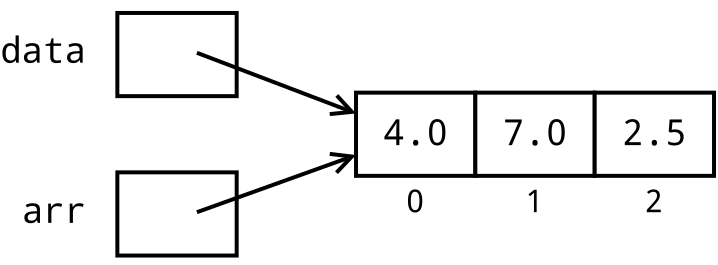
\includegraphics[scale=0.5]{figs/ch07/pass_to_array1.png}
\caption{Variable \java{arr} is a copy of the reference variable \java{data}}
\label{fig.passArray1}
\end{center}
\end{figure}

When the loop ends, the elements in the array have all changed, as show in Figure~\ref{fig.passArray2}.

\begin{figure}[!h]
\begin{center}
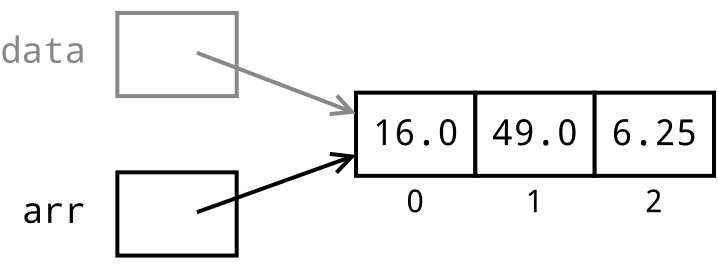
\includegraphics[scale=0.5]{figs/ch07/pass_to_array2.png}
\caption{\java{arr} refers to updated array contents}
\label{fig.passArray2}
\end{center}
\end{figure}

When method \java{squareArray} ends, its stack frame goes away and we are left with \java{data} referring to the changed array, as shown in Figure~\ref{fig.passArray3}.

\begin{figure}[!h]
\begin{center}
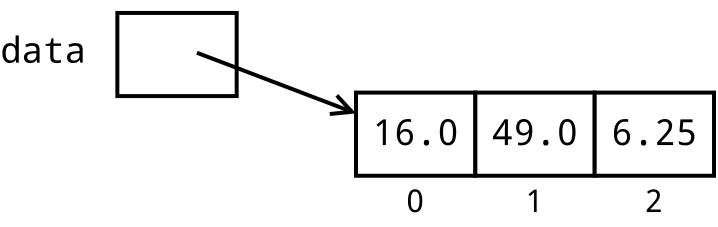
\includegraphics[scale=0.5]{figs/ch07/pass_to_array3.png}
\caption{Variable \java{data} refers to changed array contents}
\label{fig.passArray3}
\end{center}
\end{figure}

When you pass an array to a method, you get a copy of the {\em reference}. Your methods can modify the contents of the array via the reference.

Why does Java pass a copy of the reference instead of a copy of the contents? Because back when Java was invented, CPUs were slow and memory was limited. Copying the four- or eight-byte memory address of a thousand-element array is much faster than copying all thousand elements. That's the good news.

The bad news is that you can change an array's contents inadvertently. In the preceding example, once you call \java{squareArray}, your original data is gone. If you call \java{squareArray} again, you end up with the elements of the original array to the fourth power!

\section{Returning Arrays from Methods}

We're no longer working in a ``scarcity model,'' where every byte and microsecond is precious. Nowadays, CPUs are fast enough and memory plentiful enough that it makes sense to return a new array from a method, leaving the original untouched.

Consider this revised code, with line numbers for reference:

\begin{code}
 1 import java.util.Arrays;
 2
 3 public static void main(String[] args) {
 4     double [] data = {4.0, 7.0, 2.5};
 5     double [] squaredData = newSquareArray(data);
 6     System.out.println(Arrays.toString(data)); 
 7     System.out.println(Arrays.toString(squaredData));
 8 }
 9
10 public static double[] newSquareArray(double[] arr) {
11     double[] result = new double[arr.length];
12    
13     for (int i = 0; i < arr.length; i++) {
14         result[i] = arr[i] * arr[i];
15     }
16     return result;
17 }
\end{code}

Notice the return type in line 10: the method returns an array of \java{double}---the square brackets indicate an array.

When line 5 calls \java{newSquareArray}, line 11 creates a reference named \java{result} that refers to a new array with the same length as the original array. The loop changes the value in \java{result}, leaving the argument \java{arr} unmodified. Figure~\ref{fig.returnArray1} shows the memory diagram at the end of the loop.

\begin{figure}[!h]
\begin{center}
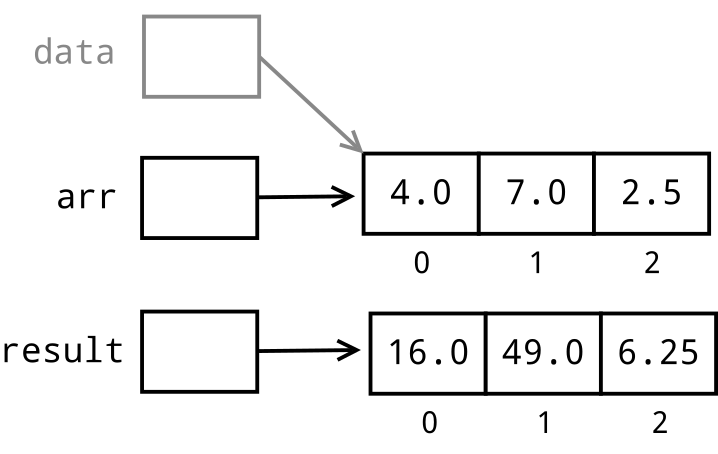
\includegraphics[scale=0.5]{figs/ch07/return_array1.png}
\caption{\java{arr} and \java{result} refer to different arrays}
\label{fig.returnArray1}
\end{center}
\end{figure}

In line 16, the method returns \java{result}, which, again, is a reference to the squared values. The return value is stored in \java{squaredData} on the left side of the assignment in line 5.  Figure~\ref{fig.returnArray2} shows the memory diagram after line 5.

\begin{figure}[!h]
\begin{center}
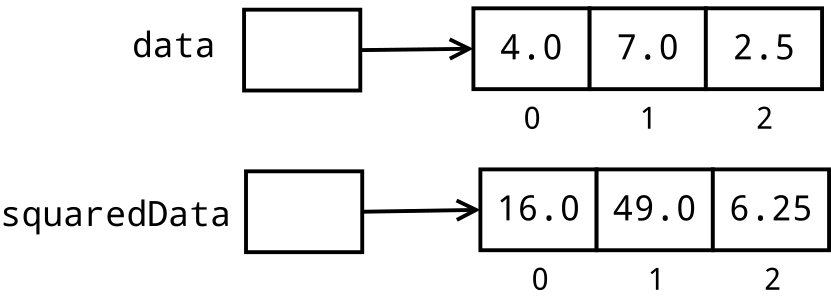
\includegraphics[scale=0.5]{figs/ch07/return_array2.png}
\caption{\java{data} and \java{squaredData} refer to different arrays}
\label{fig.returnArray2}
\end{center}
\end{figure}

So, which should you do? Update arrays in place (as in the first example) or return new arrays (as in the second example)?  There is a programming paradigm called {\em functional programming} that strongly prefers the second approach. From a functional programming standpoint, the ability to change an array in place is bad style at best and a dangerous source of programming errors at worst. In my opinion, and this is {\em only an opinion}, I agree with that viewpoint. As a guideline (not a rule), I suggest that you write your programs to return new arrays rather than modifying array arguments. However, if you are programming in an environment where memory is at a premium and programs run on slow processors, as can happen when you are programming embedded systems (\url{https://en.wikipedia.org/wiki/Embedded_system}), then saving space and time by modifying the array may be the better approach.

In the following exercises, you will be writing some methods that update an array in place and others that return a new array. This will let you practice both approaches.

\section{Exercises}

\begin{exercise}
Write methods named \java{getMax} and \java{getMin} that take an array of integers as their parameters and return the largest and smallest values in the array. Presume that the array has at least one element, and use a loop to traverse the elements.  {\em Hint:} Set the return value to the first element of the array before you enter the loop. This guarantees that your return value will be an element in the array.

Write a \java{main} method to test \java{getMax} and \java{getMin}. For example:

\begin{stdout}
Enter array length: 6
Enter 6 integers separated by spaces: 47 505 10 66 11 217
Minimum value: 10
Maximum value: 505
\end{stdout}

\end{exercise}

\begin{exercise}
The {\em Think Java} book has code to generate a histogram of scores from 0-100. In this exercise, you will generalize this to a method that accepts an array of integers as its parameter and displays the histogram.  The method is declared as:

\begin{code}
public static void displayCounts(int[] values,
     int categories, int min, int max)
\end{code}

\begin{itemize}
\item \java{values} an array of integers with the values whose histogram you want
\item \java{categories} how many ``bars'' the histogram has
\item \java{min} the minimum value of the histogram categories
\item \java{max} the maximum value of the histogram categories
\end{itemize}

For example, given this array and these calls:

\begin{code}
int[] data =  {35, 37, 19, 45, 49, 68, 95, 7, 5, 82, 84};
displayCounts(values, 5, 0, 100);
System.out.println("-----------");

// use getMin and getMax methods from preceding exercise
displayCounts(values, 4, getMin(values), getMax(values));
\end{code}

Generates this output:

\begin{stdout}
0-19: 3
20-39: 2
40-59: 2
60-79: 1
80-100: 3
-----------
5-26: 3
27-48: 2
49-70: 2
71-95: 4
\end{stdout}

You have to do some extra work to make sure that the maximum value is included in the output of the last category range. Notice, for example, in the first histogram, all the categories have a range of 20 except the last, which has a range of 21.
\end{exercise}

\begin{exercise}
\label{ex:standardize}
Write the following methods, each of which takes an array of \java{double} values as a parameter:

\begin{itemize}
\item The \java{mean} method returns the arithmetic mean (average) of the array elements.

\item The \java{stdev} method returns the standard deviation of the array elements, using this formula
\begin{equation*}
s = \sqrt {{n \sum{x_i} ^2 - \left(\sum{x_i}\right)^2} \over {n (n - 1)}}
\end{equation*}

where $n$ is the number of items in the array, $\sum{x_i} ^2$ is the sum of the squares of the individual items, and $\left(\sum{x_i}\right)^2$ is the square of the total of all the items in the array.

\item The \java{standardize} returns a new array of the values converted to {\em standard scores}. First, calculate the mean $m$ and standard deviation $s$ of the entries in the original array. Each entry in the result array will be \java{(arr[i] - m) / s}. This method must call the \java{mean} and \java{stdev} methods.

Write a \java{main} method to test the \java{standardize} method. For example, an array with values
\java{\{47.0, 11.0, 10.0, 66.0, 8.5\}} will generate these standard scores: \java{\{0.700, -0.662, -0.700, 1.418, -0.756\}} (to three decimal places). 

\end{itemize}
\end{exercise}

\begin{exercise}
\label{ex:stringReversal}

Unlike the string reversal method shown in {\em Think Java}, where a program built a new string that had its characters in the reverse order of the original, in this exercise you will write a \java{void} method named \java{reverseInPlace} that takes an array of integers as its parameter and reverses the order of the items in the array--in place. In other words, you won't create a new array; you will change the order of the items within the array itself.

Write a \java{main} method that will test the method by reversing and displaying:

\begin{enumerate}
\item An empty array with no elements
\item An array with one element
\item An array with an even number of elements (more than two elements)
\item An array with an odd number of elements (more than three elements)
\end{enumerate}

To make your job easier, you might want to create a ``helper method'' named \java{reverseAndDisplay} that prints the array, calls \java{reverseInPlace} and prints the array (which should now be reversed).
\end{exercise}

\begin{exercise}
\label{ex:vectors}

You can use an array of three \java{double} values to represent a {\em vector} in three-dimensional space. The first element represents the vector's $x$-component, the second its $y$ component, and the third its $z$ component, written as $(x, y, z)$. Write a program that has these methods, each of which takes two three-element arrays as parameters:
\begin{itemize}
\item \java{add}: Returns a vector (an array of length three) representing the sum of the parameters. The sum of $(x_1, y_1, z_1)$ and $(x_2, y_2, z_2)$ is the vector $(x_1 + x_2, y_1 + y_2, z_1 + z_2)$
\item \java{dotProduct}: Returns the {\em dot product} of the parameter vectors. The dot product of  $(x_1, y_1, z_1)$ and $(x_2, y_2, z_2)$ is calculated as $x_1\cdot x_2 + y_1\cdot y_2 + z_1\cdot z_2$ 
\item \java{distance}: Returns the distance between the vectors $(x_1, y_1, z_1)$ and $(x_2, y_2, z_2)$ using the formula $\sqrt{(x_1 - x_2)^2 + (y_1 - y_2)^2 + (z_1 - z_2)^2}$
\end{itemize}

The \java{main} method will ask the user to enter two vectors and then display the sum, dot product, and distance between the vectors. To avoid repetitious code, you might want to write a \java{getVector} method that has a prompt and a \java{Scanner} as its parameters. This method will prompt the user for the three vector components and return an array of three \java{double} values.

Here is an example of what the program might look like:

\begin{stdout}
Enter components of the first vector,
separated by spaces: 2 1.5 4.1
Enter components of the second vector,
separated by spaces: 7 3.5 1.2
Sum of vectors: (9.000, 5.000, 5.300)
Distance between vectors: 6.116
Dot product of vectors: 24.170
\end{stdout}

\end{exercise}

\begin{exercise}
In this exercise, you will find the correlation between the elements in two arrays of equal length.
Your program will ask the user for the number of entries in each array, read them in, and see how good a linear relationship they have to each other by calculating the {\em correlation coefficient}. This is a number that ranges from 1.0 (the two arrays are perfectly related to each other) to -1.0 (the arrays are perfectly inversely correlated to one another---as an example, think of the heights of the two ends of a seesaw in motion). A correlation of zero means the values in the two arrays have no linear relationship.

Write a method named \java{correlation} that takes two arrays of double and returns the correlation coefficient $r$ according to this formula:

\begin{equation*}
%r = {{\sum x_iy_i - \left(\sum x_i \sum y_i \over n\right)} \over {(n - 1) s_x s_y}}
r = {{n \sum x_iy_i - (\sum x_i)(\sum y_i)} \over {\sqrt {\left[n \sum x_i^2 - (\sum x_i)^2\right]\left[n \sum y_i^2 - (\sum y_i)^2\right]}}}
\end{equation*}

Here is an example of what the output might look like. The data are people's height in centimeters for the first array and their weight in kilograms for the second array.

\begin{stdout}
Enter number of elements in each array: 5
Enter the 5 elements in the first array: 178 176 160 180 186
Enter the 5 elements in the second array: 84.2 77.3 60 65.5 82.1
The correlation coefficient is 0.710.
\end{stdout}

\end{exercise}

\begin{exercise}
Write a method called \java{separate} which takes an array of integers as its argument and returns a new array that consists of all odd elements in the first array followed by all the even numbers in the first array, in the same relative order.

This method will require two passes (traversals) through the array.

Then, write a \java{main} method to test the \java{separate} method. Here is what it
might look like:

\begin{stdout}
Enter number of items in array: 6
Enter the items, separated by spaces: 10 47 11 66 5 98
Array with odd, then even elements: [47, 11, 5, 10, 66, 98]
\end{stdout}

You may use the \java{java.utils.Arrays.toString} method to print the result array. Make sure you test your program with an array that contains only odd numbers and again with only even numbers.

\end{exercise}

